\begin{figure*}[tb]
	%\centering
	\begin{subfigure}[b]{\columnwidth}
		%\centering
		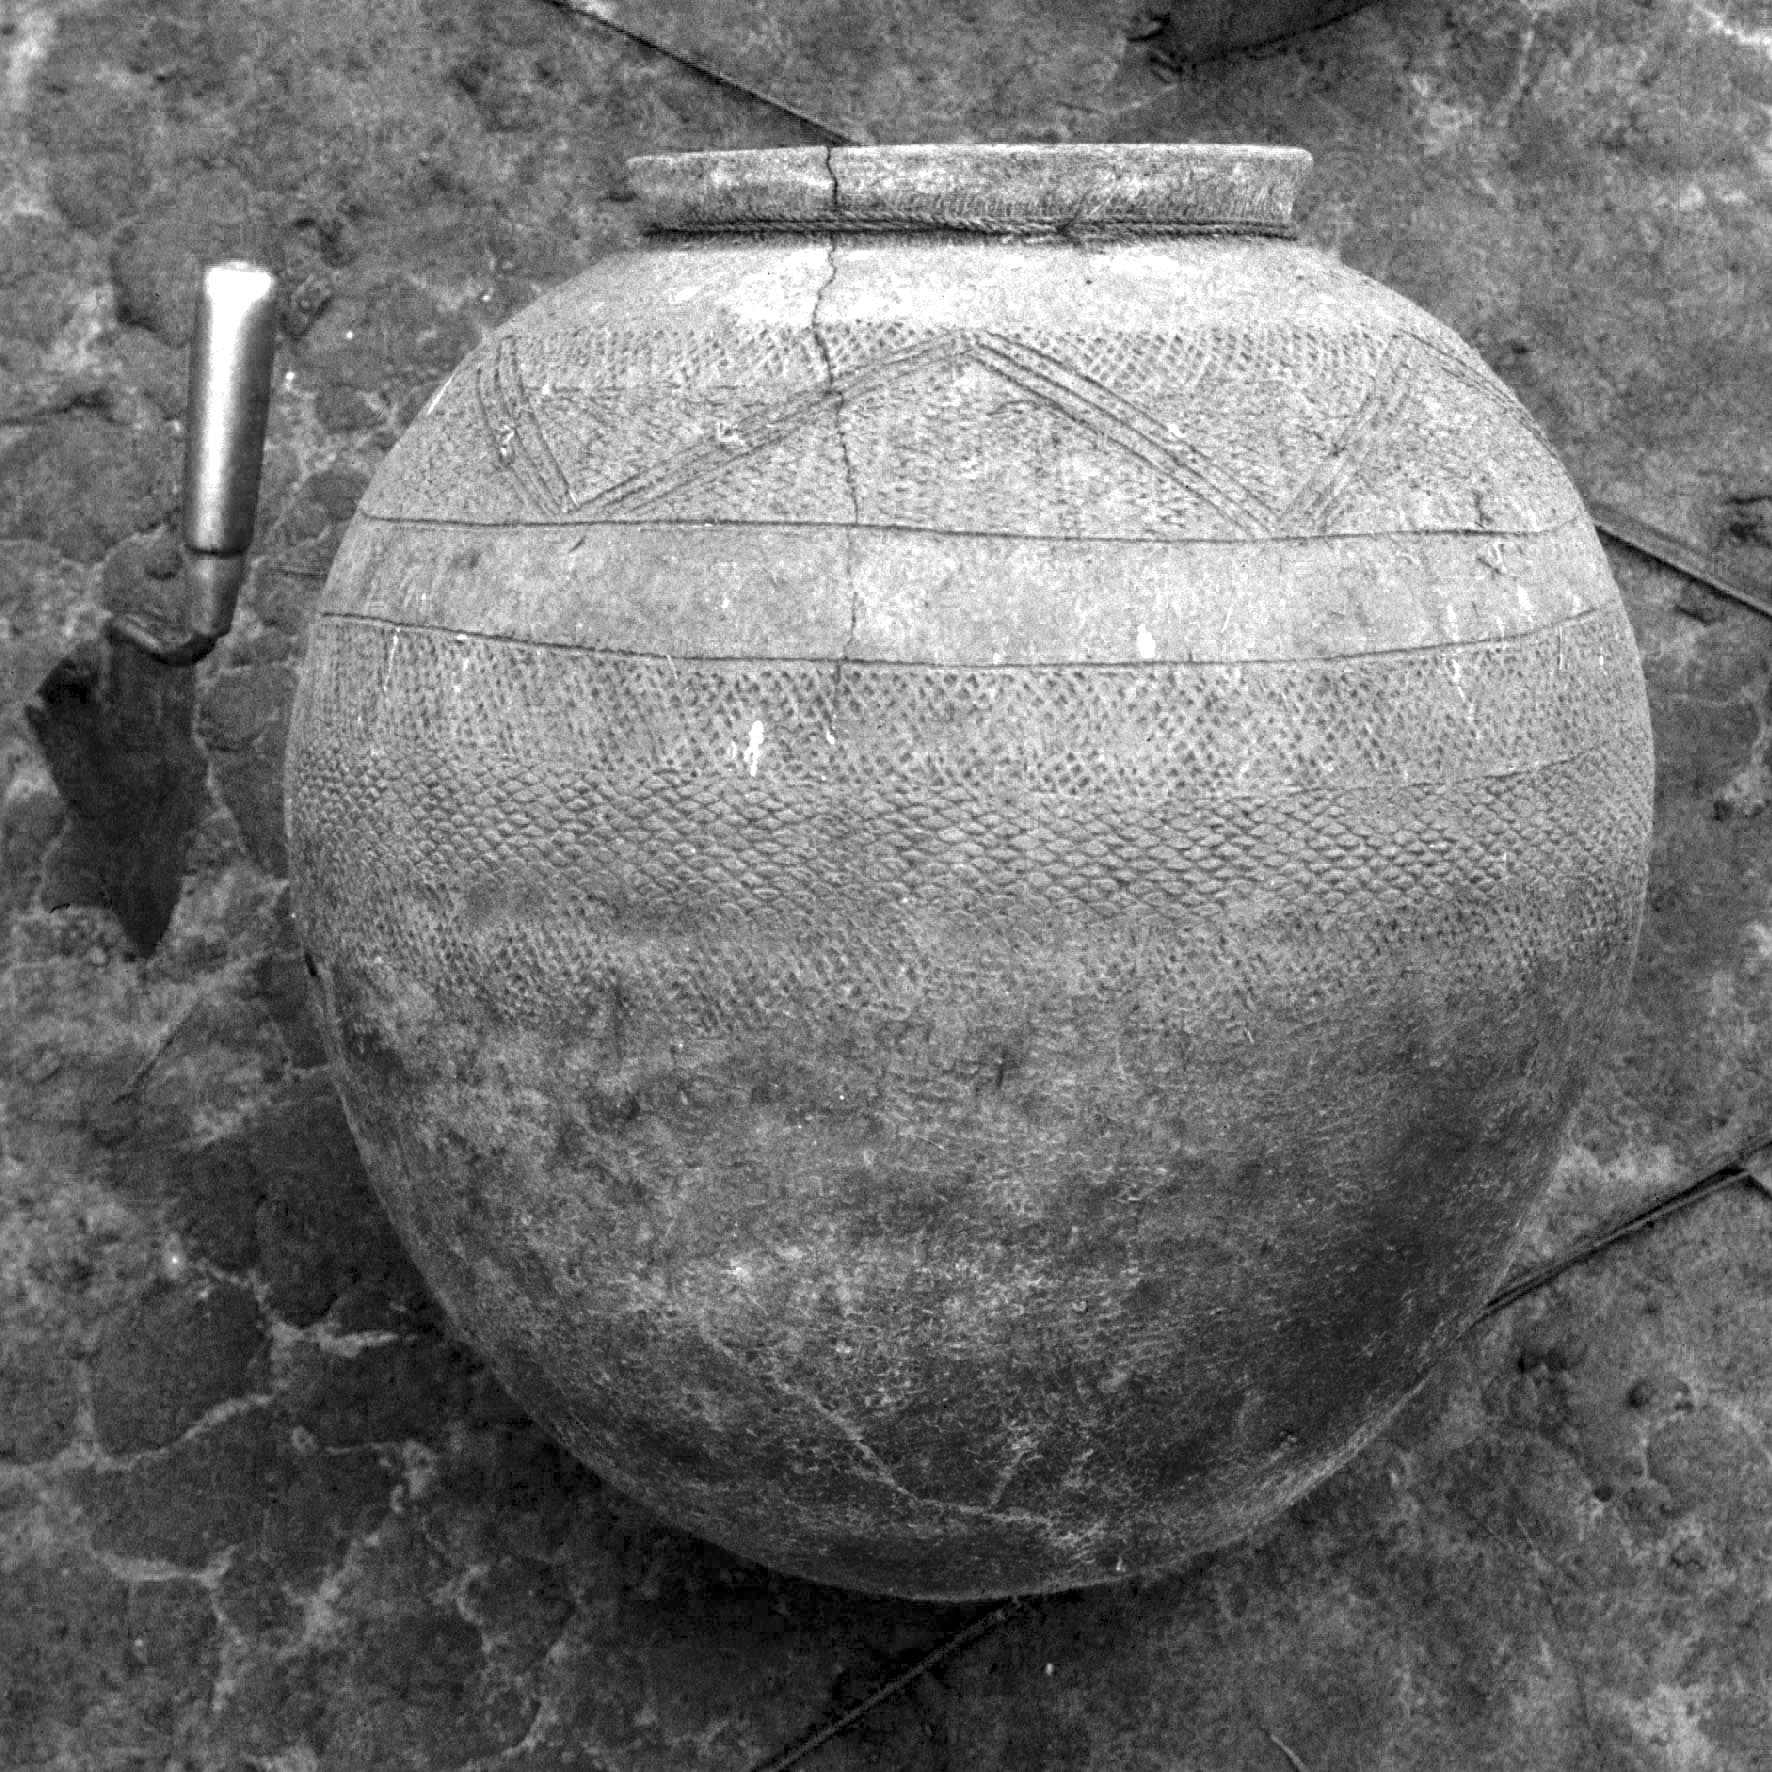
\includegraphics[width=\columnwidth]{fig/KPT85-101_Gef_E85-024-9.jpg}
		\caption{Gefäß mit konvexer Wandung und kurzem, ausbiegendem Rand (Foto: M. K. H. Eggert, 1985).}
		\label{fig:KPT85_Foto-Gef}
	\end{subfigure}\hfill
	\begin{subfigure}[b]{\columnwidth}
		%\centering
		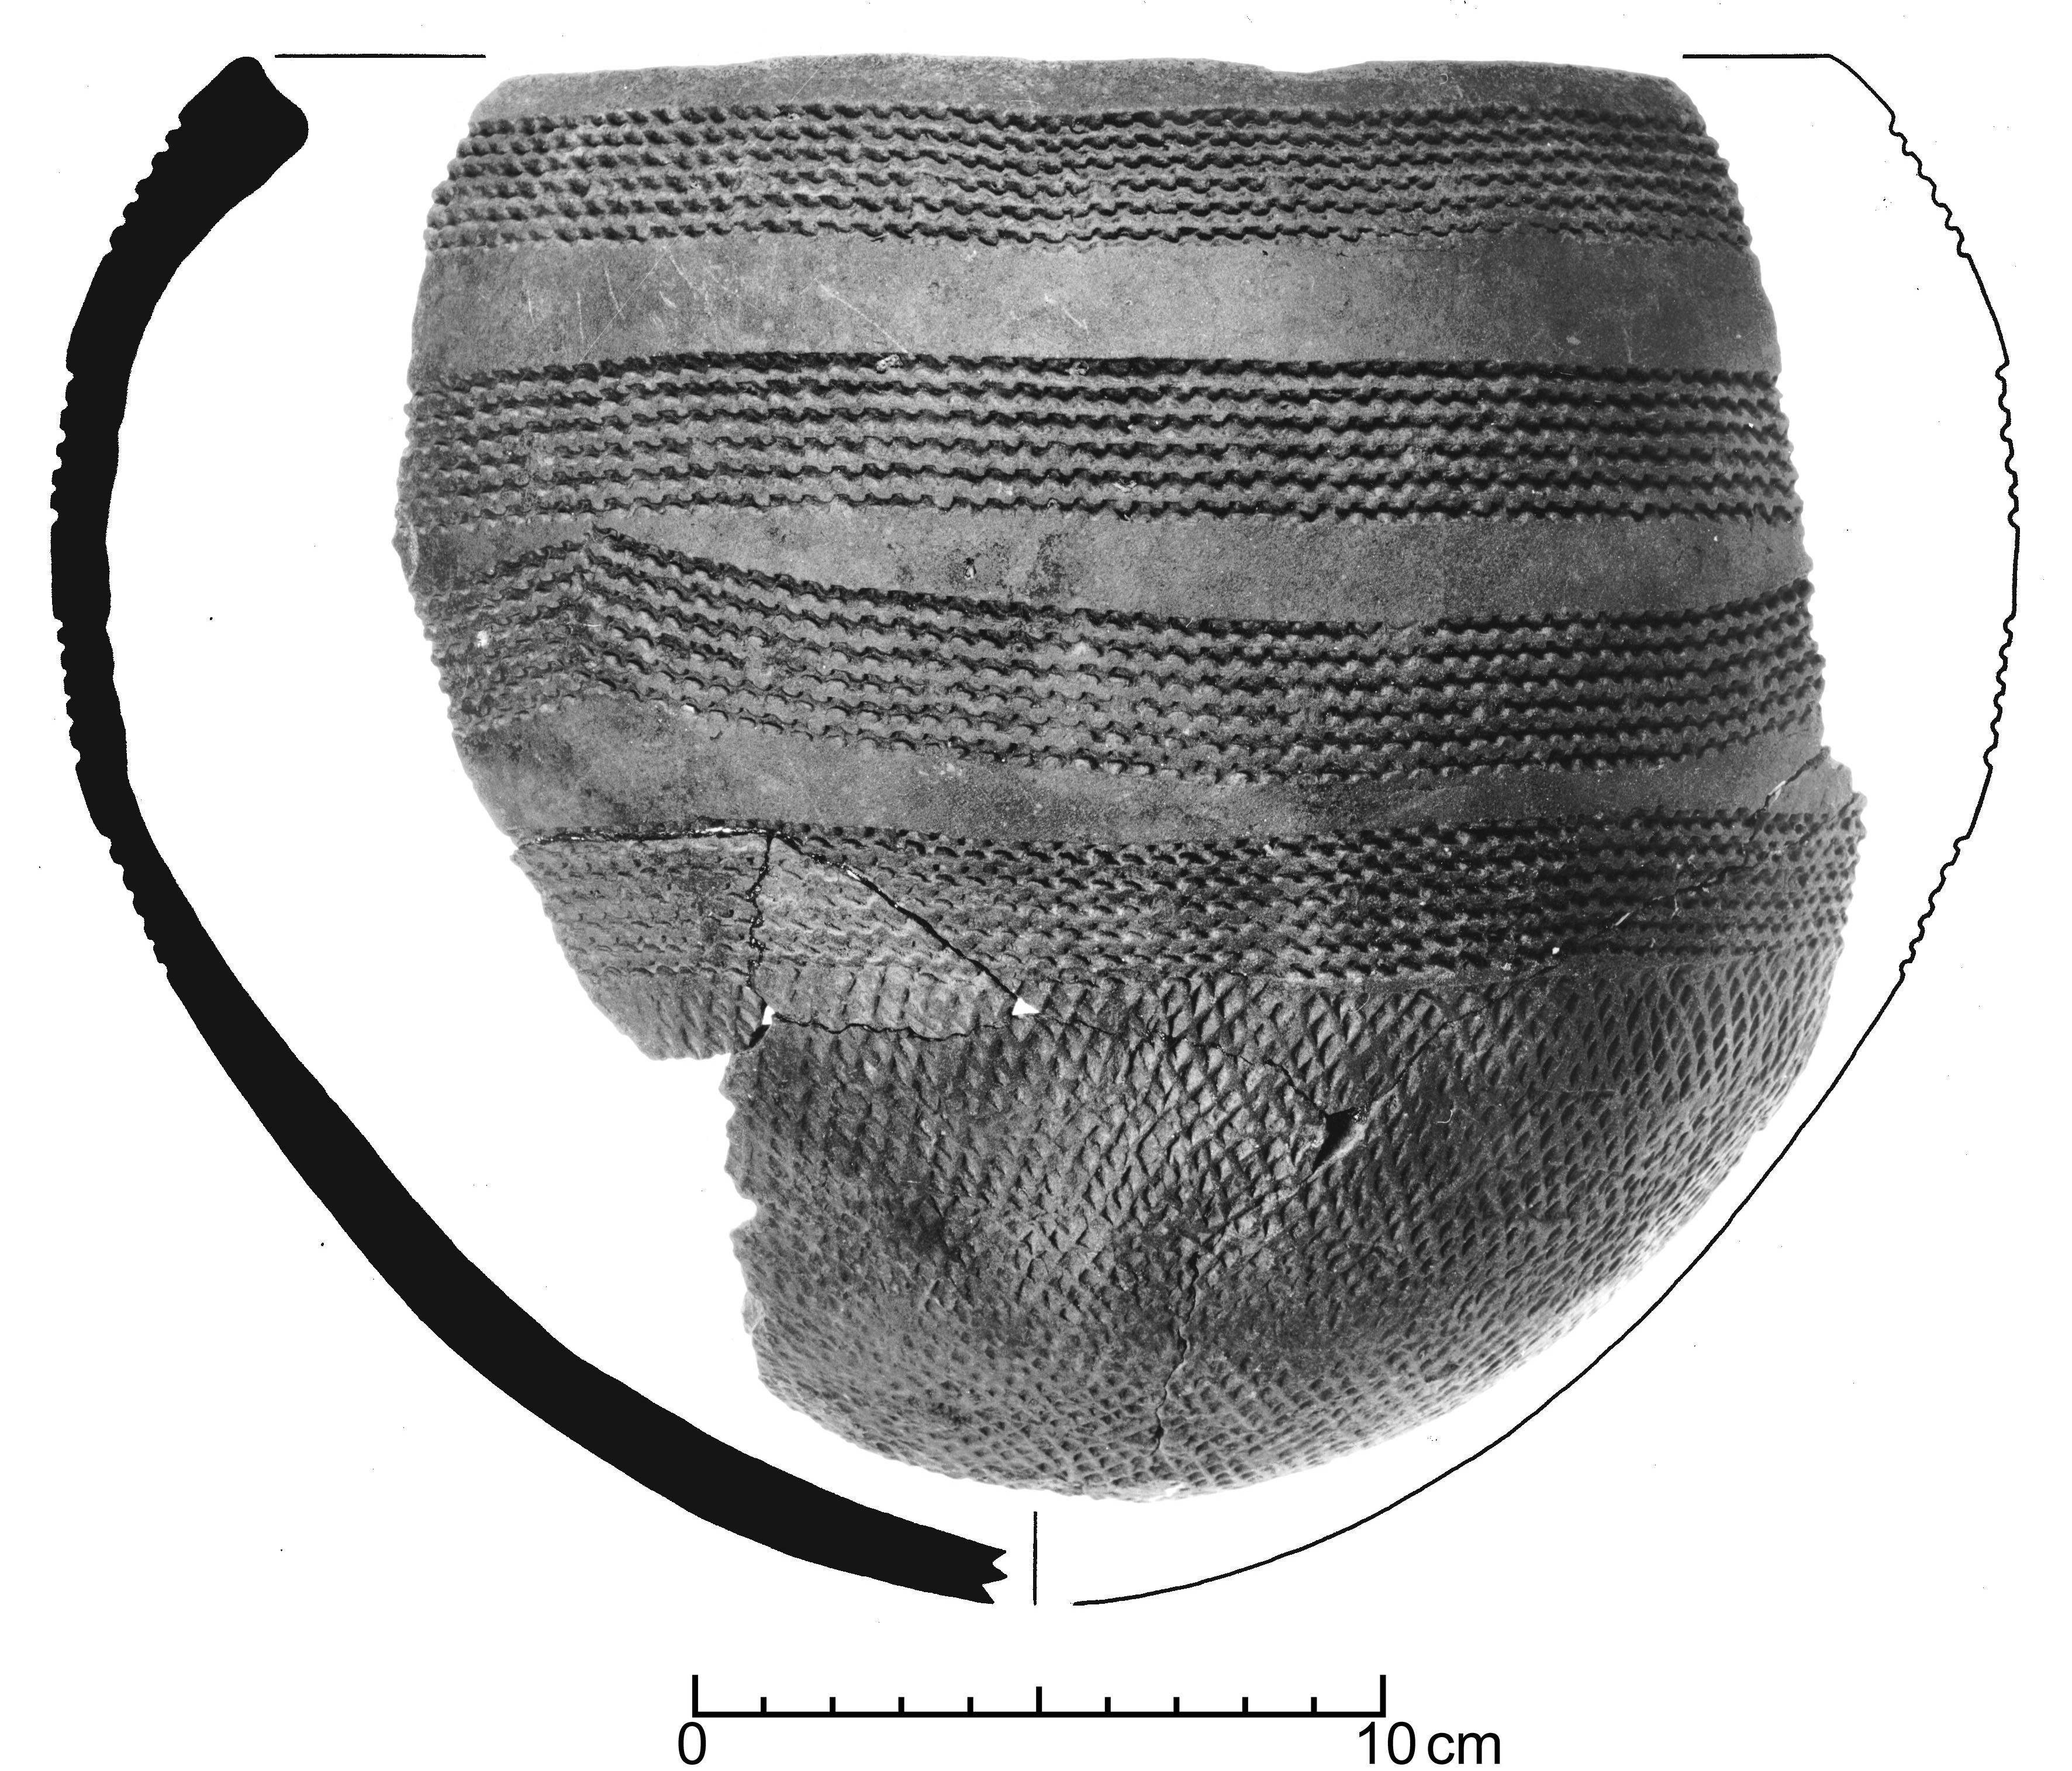
\includegraphics[width=\columnwidth]{fig/KPT85-101-10_M1-2_M.jpg}
		\caption{Schalenförmiges Gefäß mit konvexer Wandung und einbiegendem Rand (H1; Taf.~22.1).}
		\label{fig:KPT85-101-Gef}
	\end{subfigure}
	\caption{Kpetene (Fpl.~220): Gefäße der Kpetene-Gruppe.}
	\label{fig:KPT85_Typvertreter}
\end{figure*}

\subsubsection{Kpetene-Gruppe}\label{sec:KPT-Gr}

Die Kpetene-Gruppe umfasst wenige rouletteverzierte Gefäße und Gefäßfragmente, die am oberen \mbox{Ubangi} gefunden wurden (Abb.~\ref{fig:KPT_Verbreitung}). Lediglich acht GE konnten der Stilgruppe zugewiesen werden, wobei in lediglich drei Fällen eine Zuweisung zweifelsfrei möglich war. Daher kann im Fall der Kpetene-Gruppe auch nicht von einer Stilgruppe im engeren Sinne gesprochen werden. Die aus mehreren Schnitzroulette-Bändern bestehende Verzierung grenzt die hier entsprechend zusammengefassten Stücke jedoch ebenso deutlich wie die auffällig Glimmer-haltigen \textit{Fabrics} von den sonstigen rezenten Töpfereierzeugnissen am oberen \mbox{Ubangi} ab (Kap.~\ref{sec:DAM-Gr}--\ref{sec:BAN-Gr}). Die wenigen Stücke weisen neben Gemeinsamkeiten durchaus eine interne Variation auf und die zu beobachtende Verbreitung (Abb.~\ref{fig:KPT_Verbreitung}) legt nahe, das es sich nicht um ein auf einen einzelnen Platz isoliertes Phänomen handelt (siehe Kap.~\ref{sec:SHG-LKW_Einzelfunde}). Die Kpetene-Gruppe ist folglich, auch mit Blick auf die Möglichkeit, dass ein verbesserter Forschungsstand in der Zukunft eine umfassendere Definition zulässt, als Provisorium konzipiert und hier aus Gründen der terminologischen Einheitlichkeit im Detail beschrieben.\footnote{Siehe Anm.~\ref{ftn:ProvisorischeStilGr}.}

\paragraph{Technologische Merkmale}\hspace{-.5em}|\hspace{.5em}%
Die wenigen Stücke der Kpetene-Gruppe zeichnen sich durch einen Scherben aus, der größere Anteile nichtplastischer Partikel der Korngrößen \textit{coarse} und \textit{very coarse} enthält. Regelhaft handelt es sich um Quarzsand sowie Glimmer und ausgebrannte Organik. In zwei Fällen konnten auch geringe Anteile Schamott in den Scherben beobachtete werden. Die genutzten Tone sind häufig rotbrennend, nur eine GE deutet die Nutzung weißbrennender Tone an. Die Oberflächen der Scherben sind häufig geglättet.

\paragraph{Formen}\hspace{-.5em}|\hspace{.5em}%
Vier der Kpetene-Gruppe zugewiesenen GE sind rund- bis spitzbodige hohe schalenförmige Gefäße mit einbiegenden Rändern (Typ H1; Abb.~\ref{fig:KPT85-101-Gef}). Bei zwei weiteren GE blieb unklar, ob es sich um eine eher flache Variante der gleichen Grundform handelt (Typ H2). Eine Ausnahme bildet ein am eponymen Fundplatz Kpetene fotografiertes Gefäß (Abb.~\ref{fig:KPT85_Foto-Gef}). Es handelt sich um ein rundbodiges, stark bauchiges Gefäß ohne ausgeformten Halsbereich, das über einen kurzen, leicht ausbiegenden Rand verfügt (D2). Mit den anderen GE der Kpetene-Gruppe hat es die langovale Grundform mit rundem Boden und eine aus mehreren Bändern bestehende Rouletteverzierung gemein.

Die rund- bis spitzbodigen Schalen der Kpetene-Gruppen zeigen regelmäßig einbiegende Ränder (C3; Abb.~\ref{fig:KPT85-101-Gef}). Lediglich das fotografierte Gefäß verfügt über einen kurzen, ausbiegenden Rand (B1; Abb.~\ref{fig:KPT85_Foto-Gef}). Die Mündungen sind regelmäßig schräg nach innen abgestrichen (M6). Zwei GE weisen gerillte Randlippen auf (M4).

Lediglich bei einer GE konnte die Form des Bodens beobachtet werden. Es handelte sich um einen leicht spitzen Rundboden. Die fotografierte GE aus Kpetene zeigt ebenfalls einen runden, leicht spitz zulaufenden Boden (Abb.~\ref{fig:KPT85_Foto-Gef}).

\begin{figure*}[p]
	\centering
	\includegraphics[width=\textwidth]{fig/KPT_Verbreitung.pdf}
	\caption{Kpetene-Gruppe: Verbreitung.}
	\label{fig:KPT_Verbreitung}
\end{figure*}

\paragraph{Verzierungen}\hspace{-.5em}|\hspace{.5em}%
Durch die Nutzung verschiedener Verzierungstechniken werden die dem Kpetene-Stil zurgerechneten Gefäße regelhaft in einen unteren sowie einen oberen Teil untergliedert. Während der untere Teil flächigen Mattenabdruck (Tab.~\ref{tab:Verzierungselemente}: 12) zeigt, weist der obere Teil horizontale, alternierende Bänder aus Schnitzroulette auf (Abb.~\ref{fig:KPT85_Typvertreter}). Die gebänderte Verzierung der Gefäßoberteile kann neben verschiedenen Schnitzroulette-Variationen auch Ritzverzierungen umfassen (Abb.~\ref{fig:KPT85_Foto-Gef}). Eine GE weist drei mit dem gleichen \mbox{Roulette} gefertigte horizontale  Bänder sowie ein bogenförmiges, girlandenartiges Band auf (Abb.~\ref{fig:KPT85-101-Gef}).

Diagnostisches Merkmal der Kpetene-Keramik sind die verschiedene Formen von Schnitzrouletteverzierung. Vegetabilisches \mbox{Roulette} wurde in keinem Fall beobachtet. Das Schnitzroulette findet sich ohne Ausnahme auf den oberen Gefäßteilen, auf dem Bauch sowie im Schulterbereich der Gefäße. Nur eine GE zeigt auch Schnitzroulette auf dem Rand. In seltenerem Maße treten auch horizontale Rillen auf (Tab.~\ref{tab:Verzierungselemente}: 02.1; 15\,\%). Sehr viel seltener lassen sich im Material horizontale Bänder aus feinen Eindrücken beobachten (Tab.~\ref{tab:Verzierungselemente}: 04.16; 8\,\%; Abb.~\ref{fig:KPT85-101-Gef}).

\paragraph{Datierung}\hspace{-.5em}|\hspace{.5em}%
Für die innerhalb des Kpetene-Stils subsumierten keramischen Formen liegen keine absoluten Datierungen vor. Jedoch unterstreicht die Beobachtung eines noch in Benutzung befindlichen Gefäßes am eponymen Fundplatz Kpetene (Fpl. 220; Abb.~\ref{fig:KPT85_Foto-Gef}) am oberen \mbox{Ubangi} zum Zeitpunkt der Befahrung im Jahr 1985 den rezenten Charakter des entsprechenden Materials. Mit Blick auf die Schnitzroulette-Bänder zeigt das Material gewisse Ähnlichkeiten zu jener Keramik, die im Westen der Zentralafrikanischen Republik, in Nana-Modé ausgegraben wurde \parencite[34 Abb.~7,1,3--6]{David.1977}. Auch dieses Material umfasst Gefäße mit horizontalen sowie girlandenartigen Schnitzroulettebändern. Das Material der Kpetene-Gruppe setzt sich von der rezenten, schnitzrouletteverzierten Keramik der Dama-Gruppe (Kap.~\ref{sec:DAM-Gr}) sowohl durch seine ornamentalen (flächige anstatt lediglich einzelne Bänder im Schulterbereich) als auch seine morphologischen Eigenheiten (spitzbodige hohe  Gefäßtypen) ab. Von der ebenfalls rezenten Mbati-Ngombe-Keramik (Kap.~\ref{sec:MBN-Gr}), die ähnliche Gefäßformen zeigt, unterscheidet sie sich durch die Verwendung von Schnitz- anstatt vegetabilischer Roulette.

\paragraph{Verbreitung}\hspace{-.5em}|\hspace{.5em}%
Das Material der Kpetene-Gruppe wurde an fünf Fundplätzen entlang dem oberen \mbox{Ubangi}, stromauf von Bangui gefunden (Abb.~\ref{fig:KPT_Verbreitung}). Zweifelsfrei zuweisbare Stücke fanden sich lediglich in der namensgebenden Fundstelle Kpetene (Fpl.~220), in Gbandami (Fpl.~226) und in Kouango (Fpl.~229). 